\documentclass[12pt]{article}
\usepackage[T1]{fontenc}
\usepackage[utf8]{inputenc} %utf8 % lettere accentate da tastiera
\usepackage[italian]{babel} % lingua del documento
\usepackage{lmodern}
\usepackage[hidelinks]{hyperref}
\usepackage{graphicx}
\usepackage{lmodern}
\usepackage{amssymb}
\usepackage{enumitem}
\usepackage{lmodern}  % for bold teletype font
\usepackage{amsmath}  % for \hookrightarrow
\usepackage{xcolor}   % for \textcolor
\usepackage{listings}
\usepackage{float}
\usepackage{cleveref}
\lstset{
  basicstyle=\ttfamily,
  columns=fullflexible,
  frame=single,
  breaklines=true,
  postbreak=\mbox{\textcolor{red}{$\hookrightarrow$}\space},
}

\frenchspacing

\graphicspath{ {./img/} }

% nested enumerations
\renewcommand{\labelenumii}{\theenumii}
\renewcommand{\theenumii}{\theenumi.\arabic{enumii}.}


\begin{document}
\pagenumbering{roman}
\begin{titlepage}

\begin{center}
\textsc{Università degli Studi di Milano-Bicocca}\\
\textsc{Dipartimento di Informatica, Sistemistica e Comunicazione}\\
\end{center}
\begin{figure}[h]
\centering

\includegraphics[width=0.3\linewidth]{img/logo_unimib.pdf}
\end{figure}



\vspace*{\stretch{3}}
\begin{center}
\begin{Huge}
%TITOLO
\LARGE{-- Progetto Sistemi Complessi --}\\
\textbf{Supermarket Queue}\\

\end{Huge}

\end{center}\par

\vspace*{\stretch{3}}


\par
\vspace*{\stretch{1}}
\begin{flushright}
\textsc{
Francesco Stranieri 816551\\
Davide Marchetti 815990\\
Mattia Vincenzi 860579}\\
\end{flushright}
\vspace*{\stretch{3}}
\centering
Anno Accademico 2019 - 2020\par
\end{titlepage}


\cleardoublepage %inserisce una pagina totalmente bianca

\hypersetup{linkcolor=black}
\tableofcontents

\newpage
\pagenumbering{arabic}
\setcounter{page}{1}

\section{Introduzione}

% Riprendere Abstract e dare un idea di quello che abbiamo fatto. Introdurre la struttura della relazione. 
\section{Supermarket Model}

\subsection{Struttura}
La struttura del supermercato viene caricata tramite un apposito file \lstinline{txt}. 
Tale file è strutturato in modo tale da fornire al modello alcune informazioni essenziali.

La prima riga prevede la dimensione del supermercato.
In questo studio si è deciso di modellarne uno di medie dimensioni, con un'area totale pari a $32x30$.

Sulla seconda riga sono presenti due variabili dipendenti dall'area, ossia la capienza massima e il numero di riga entro il quale un agente può cambiare cassa. 
Questo risulta essere particolarmente importante per limitare l'effetto "sciame", il quale si verifica, nella modalità Classic, quando più agenti provano contemporaneamente a cambiare cassa. Limitandone l'effetto, le code risultano più ordinate.
Nel nostro studio, quest'ultimo parametro ha un valore pari a $10$ mentre la capienza massima è stata impostata a $35$.

La terza riga descrive la tipologia di coda implementata dalla mappa. 
Sono presenti infatti due tipi di coda, Classic e Snake, come descritto nella Sezione \ref{}.

Infine, nelle restanti righe, è presente la struttura vera e propria della mappa. 
Il simbolo \texttt{'X'} corrisponde ad un ostacolo, la \texttt{'O'} alle celle percorribili da un agente. 
I numeri da \texttt{1} a \texttt{N} equivalgono alle casse, mentre le lettere da \texttt{A} a \texttt{Z} corrispondono ai punti di spawn. 
Questi sono necessari in quanto la fase di shopping, che vede l'agente muoversi tra gli scaffali con l'obiettivo di acquistare un certo numero di prodotti, viene interpretata dal nostro modello come una black-box. 
Pertanto risulta inevitabile predisporre, in concomitanza di ogni scaffale, un'apposita cella che permette all'agente di raggiungere una determinata cassa, dopo essere stato spawnato. 
Tale argomento verrà trattato nella Sezione \ref{}.
La modalità Snake prevede inoltre due simboli aggiuntivi, ovvero la lettera \texttt{S} che indica l'ingresso nel serpentone e la lettera \texttt{Z} che indica la relativa uscita. 

La Figura \ref{} mostra il contenuto del file \lstinline{txt} usato per la modalità Classic. La Figura \ref{} mostra invece la struttura della mappa una volta caricata dal modello.

\subsection{Tipologie di Coda}
Il modello implementa due diverse tipologie di coda:
\begin{itemize}
    \item \textbf{Classic} rappresenta, per l'appunto, la modalità più classica; è quindi presente un numero di code pari al numero di casse aperte. 
    Nel nostro progetto una fila può avere una lunghezza massima pari a $12$ celle. 
    Questo valore permette di studiare efficacemente i fenomeni di nostro interesse. 
    \item \textbf{Snake} rappresenta invece la così detta modalità 'a serpentone'. 
    In questa modalità è presente un unico ingresso, il quale permette di percorrere l'unica fila presente fino a raggiungere la cella di uscita. Una volta raggiunta l'agente verrà assegnato alla prima cassa libera, facendo così scorrere la fila.
\end{itemize}
E' importante sottolineare come nella modalità Classic la scelta della cassa ottimale è rimandata all'agente, mentre nella modalità Snake è l'ambiente a dover effettuare questa scelta.

\subsection{Floor Field}
La scelta della destinazione ottimale, ossia della cassa più vicina e con il minor numero di persone in coda, avviene grazie all'utilizzo dei \textit{floor fields}.
Nel dettaglio, la nostra implementazione vede la generazione di un numero di floor field pari al numero di casse aperte. 
Il corrispondente valore di ogni cella è pari alla distanza euclidea, dal punto di spawn fino alla corrispettiva cassa, descritta tramite l'equazione:
\begin{equation*}
 d\left( p,q\right)   = \sqrt {\sum _{i=1}^{n}  \left( q_{i}-p_{i}\right)^2 } .
\end{equation*}
In corrispondenza di un ostacolo la distanza è stata impostata pari a $+ \infty$.

L'agente, avendo una visione locale dell'ambiente che coincide con il suo vicinato, sceglie quindi, per ogni cassa, la destinazione locale ottima. 
A questi valori viene successivamente sommato il numero attuale di persone in coda, in modo da tener conto anche dell'affollamento.
Ora, tra tutte le destinazioni locali, viene selezionata quella ottimale, corrispondente quindi alla cassa scelta come obiettivo.
Il movimento dell'agente sarà quindi basato sulla cassa che tale agente ha come obiettivo.

\subsection{Spawn degli Agenti}
Per far sì che il modello rappresenti una situazione vicina alla realtà, si è scelto di modellare l'ingresso degli agenti in modo tale da avere una fase iniziale di graduale riempimento, fino al raggiungimento di un picco oltre il quale ci sarà un progressivo svuotamento.

Viene quindi generato, ad ogni step, un numero compreso tra $0$ e $1$ secondo la seguente equazione:
\begin{equation*}
p_1 = -\frac{\cos\left(\frac{t\pi}{1200}\right)}{2}+\frac{1}{2} .
\end{equation*}
Successivamente viene generato un numero casuale $p_2$, sempre tra $0$ e $1$. 
Se $p_2 > p_1$ allora l'agente verrà effettivamente creato.

La Figura \ref{} mostra il grafico di tale funzione. 
E' possibile notare come la probabilità relativa alla creazione di un agente tende ad aumentare fino a metà giornata, quando il numero di step è pari a $1200$. 
Superato questo valore la probabilità tenderà a scendere, garantendo così lo svuotamento del supermercato.

\subsection{Gestione delle Casse}
La gestione delle casse è stata pensata in modo tale che il numero di casse aperte risulti coerente sia con la specifica fase della giornata sia con il numero di persone presenti nel supermercato.
Questo implica che durante la fase di riempimento le casse tenderanno ad aprire. 
Durante il picco ci sarà quindi una situazione in cui tutte le casse saranno aperte, in modo da gestire efficacemente la fase di maggiore affluenza. 
Infine, durante lo svuotamento, le casse chiuderanno in maniera graduale. 

E' importante sottolineare come questa gestione non è stata implementata in maniera simmetrica ma bensì cercando di anticipare una possibile apertura, posticipando così la corrispettiva chiusura. 

\subsection{Gestione degli step}

\section{Agenti}

Gli agenti considerati nella modellazione di uno scenario rappresentante un supermercato sono diversi:

\begin{itemize}
    \item \textbf{Ostacoli} (Obstacles): rappresentano ostacoli fermi all'interno della mappa, zone non calpestabili dagli agenti in movimento.
    \item \textbf{Cassieri} (Cashiers): rappresentano i cassieri del supermercato, si posizionano alla cassa per servire i clienti, rimanendo nella loro posizione. Compaiono nello scenario quando la cassa apre e scompaiono quando la cassa chiude. Insieme a questi agenti vengono gestite le casse vere e proprie, ovvero i punti di pagamento a cui i clienti sono diretti prima di uscire dal supermercato. Queste casse rappresentano, come gli ostacoli, delle zone non calpestabili del terreno, ma contengono anche proprietà aggiuntive come il tempo per cui devono ancora rimanere aperte e lo stato attuale: aperta o chiusa. 
    \item \textbf{Clienti} (Customers): questi sono gli agenti che si muovono all'interno dell'area casse. Questi agenti possiedono diversi attributi utili all'esecuzione del proprio compito tra cui: numero di prodotti da acquistare, tempo necessario per fare la spesa, tempo di pagamento, stato attuale, prossima destinazione da raggiungere ecc...
    Nella modalità \textbf{snake} eseguono un compito molto semplice, ovvero quello di accodarsi e aspettare che gli venga assegnata una cassa una volta raggiunta la fine della coda. Nella modalità \textbf{classic}, invece, i clienti ricercano quella che è la soluzione che ritengono migliore per poter raggiungere una cassa disponibile nel minor tempo possibile, tenendo in considerazione diversi fattori tra cui la distanza da ogni cassa e il numero di persone nelle corrispondenti coda. 
\end{itemize}

Da questo momento in poi verranno analizzati quelli che sono gli aspetti più interessanti utilizzati per la gestione degli agenti. Nella trattazione successiva gli agenti considerati sono i Clienti (Customers), in quanto sono coloro che hanno la possibilità di muoversi e di accodarsi alle casse.

\subsection{Entrata all'area casse}

I clienti una volta terminata la spesa all'interno del supermercato, devono comparire nella zona casse, in modo da poter pagare e poi uscire dallo scenario. Nel supermercato modellato sono presenti 5 corsie, da ognuna delle quali si può giungere all'area casse. Lo spawn degli agenti nell'area casse viene quindi eseguito su una di queste 5 corsie, ma la distribuzione di probabilità di accedere all'area casse non sarà uniforme sulle 5 corsie in quanto sarà molto più probabile che una persona percorra tutte o quasi le corsie. Questo perché prodotti di categorie diverse sono in corsie differenti e spesso quando si va fare la spesa si ha la necessità di acquistare prodotti di vario tipo, unito al fatto che la disposizione degli scaffali e dei prodotti è simile nei vari supermercati, predeterminando il percorso dei clienti, e mostrandogli più prodotti di quelli che sarebbero inizialmente intenzionati ad acquistare. Sulla base di tali motivazioni è stata predisposta un probabilità del 35\% che un agente acceda alla zona casse dall'ultima corsia, del 25\% dalla penultima, del 20\% dalla terza ed infine del 10\% dalla seconda e dalla prima.  

\subsection{Fasi Agente}

Un cliente durante la sua permanenza all'interno del supermercato si trova in diverse fase, ad ognuna delle quali corrisponde un diverso obiettivo che l'agente deve perseguire. Naturalmente le fasi saranno leggermente differenti nelle due modalità di code. 

Nella figura sottostante vengono mostrate le fasi dell'agente nella modalità \textbf{classic}:

\begin{itemize}
    \item \textbf{Shopping}: il cliente si trova all'interno del supermercato e sta facendo la spesa. Essendo il supermercato gestito come una \textit{black-box} il cliente non viene mostrato durante questa fase, ma è conteggiato all'interno del grafico a torta che mostra la porzione di agenti in \textbf{Shopping}. Una volta che il cliente ha terminato di fare la spesa allora passa nello stato \textbf{Reaching the queue}.
    \item \textbf{Reaching the queue}: il cliente è appena comparso nella zona casse, in una delle 5 corsie, e valuta in base alla \textit{distanza} e al \textit{numero di altre persone in ogni coda} quale sia la scelta ottimale per minimizzare il tempo di attesa alle code. In questa fase si muove verso la destinazione prestabilita, avendo anche la possibilità di cambiare la propria decisione a fronte di variazioni della situazione circostante. Una volta raggiunta la coda entra nello stato \textbf{In queue}.
    \item \textbf{In queue}: in questo stato il cliente è fermo ed attende il proprio turno per essere servito. Ad ogni step l'agente si muove in avanti qualora la fila scorra e lasci libera una cella per il movimento. Una volta raggiunta la cassa corrispondente a tale coda il cliente passa nello stato di \textbf{Paying}.
    \item \textbf{Paying}: l'agente viene servito e una volta terminato il tempo di pagamento esce dalla scena.
\end{itemize}

\begin{figure}[h!]
    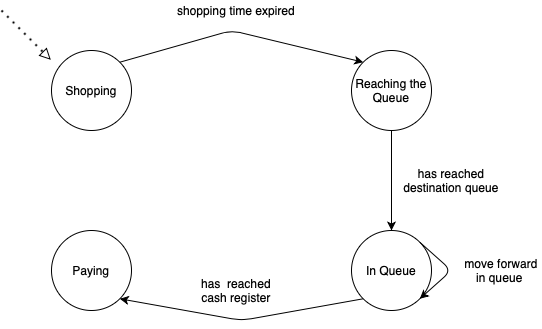
\includegraphics[width=\linewidth]{img/FSM-phases-classic.png}
    \centering
    \caption{\textit{Fasi cliente con coda \textbf{classic}.}}
\end{figure}

Nella figura sottostante vengono riportate le fasi attraversate dall'agente nella modalità \textbf{snake}. Di seguito verranno descritte solo quelle fasi che differiscono dal caso precedente:

\begin{itemize}
    \item \textbf{Shopping}.
    \item \textbf{Reaching the queue}: in questa fase il cliente si muove verso la destinazione, contrassegnata dalla posizione di inizio della coda a serpentone; una volta raggiunta la coda entra nello stato \textbf{In queue}.
    \item \textbf{In queue}: in questa fase il cliente si muove fino al fondo della coda (qualora ci siano altro agenti in attesa), e una volta raggiunta tale posizione rimane fermo in coda e si muove nel momento in cui i clienti che lo precederono muovono a loro volta in avanti. Rimane in questa fase fino al raggiungimento della posizione di fine della coda a serpentone, passando nello stato \textbf{Reaching Cashier}.
    \item \textbf{Reaching Cashier}: l'agente si trova in questa fase dal momento in cui raggiunge la testa del serpentone, mentre attende che una cassa si liberi e gli venga assegnata, fino a quando raggiunge una cassa per il pagamento (momento in cui passa nello stato \textbf{Paying}).
    \item \textbf{Paying}.
\end{itemize}

\begin{figure}[h!]
    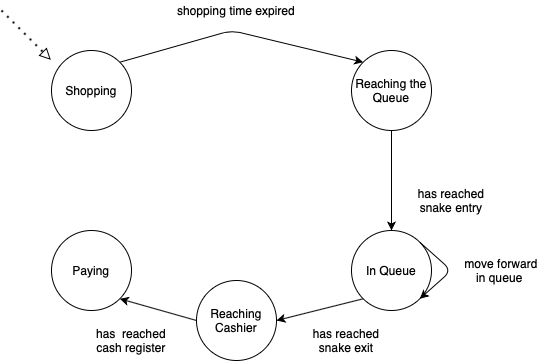
\includegraphics[width=\linewidth]{img/FSM-phases-snake.png}
    \centering
    \caption{\textit{Fasi cliente con coda \textbf{snake}.}}
\end{figure}

\subsection{Numero di Prodotti}

Un parametro importante che viene definito alla creazione dell'agente è il numero di prodotti che dovrà andare ad acquistare e che verrà utilizzato come base di partenza per il calcolo necessario a fare la spesa e per il tempo di pagamento. 

Questo parametro viene calcolato utilizzando una distribuzione normale con media e varianza espresse in funzione della capienza massima del supermercato, ovvero di 35 persone nella mappa utilizzata.

I parametri utilizzati per la normale sono $\mu = 35/2 = 17.5$ e $\sigma = 35/4 = 8.75$ scelti opportunamente dopo una fase di calibrazione e testing. 

Il numero di prodotti viene quindi ottenuto estraendo un campione da questa distribuzione normale, e arrotondandolo per eccesso, in quanto il numero di prodotti deve essere necessariamente intero.

La distribuzione ottenuta estraendo $100000$ campioni dalla normale con media e deviazione standard definiti sopra è quella riportata nella figura sottostante. 

\begin{figure}[h!]
    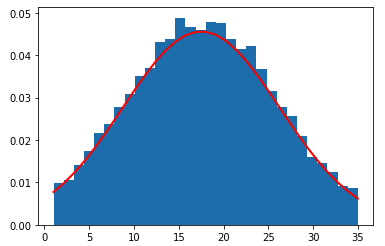
\includegraphics[width=\linewidth]{img/pcount-distribution.png}
    \centering
    \caption{Distribuzione normale con $\mu=17.5$ e $\sigma=8.75$.}
\end{figure}

\subsection{Shopping Time}

Alla creazione di un cliente, sulla base del numero di prodotti generato dalla distribuzione descritta precedentemente, viene calcolato quello che è lo \textit{shopping time}, ovvero il tempo che l'agente in questione impiegherà nella fase di \textbf{Shopping}, espresso in step. La stima di questo parametro rappresenta un'approssimazione del tempo impiegato dal cliente a fare la spesa all'interno del supermercato, ovvero dell'area da noi considerata come una \textbf{black-box}; a tal proposito l'agente non viene visualizzato nell'area casse durante questo periodo, in quanto impegnato nelle corsie del supermercato da noi non modellate. 

La formula utilizzata per calcolare questo tempo dipende dal parametro \textit{numero di prodotti} (\textit{product count}), nel seguente modo: 

\begin{equation*}
shopping time = 3 + product count * 0.75
\end{equation*}

Supponendo, ad esempio, che un cliente debba acquistare 20 prodotti, allora il tempo impiegato per fare la spesa sarà di circa 18 step.

\subsection{Paying Time}

Altro parametro che viene assegnato ad ogni cliente alla sua creazione è quello legato al tempo di pagamento (\textbf{paying time}). Questo parametro rappresenta il tempo che l'agente trascorrerà nella fase di \textbf{paying}, davanti alla cassa, in attesa di terminare il pagamento, per poi scomparire dalla scena. La stima di questo parametro rappresenta un'approssimazione del tempo impiegato dal cliente ad effettuare effettuare il pagamento; durante questo periodo il cliente sarà posizionato nella casella a fianco della cassa, in attesa di terminare il pagamento e andarsene. 

La formula utilizzata per calcolare questo tempo dipende sempre dal parametro \textit{numero di prodotti} (\textit{product count}), nel seguente modo:

\begin{equation*}
paying time = 1 + product count * 0.25
\end{equation*}

Supponendo, ad esempio, che un cliente debba acquistare 20 prodotti, allora il tempo impiegato per effettuare il pagamento una volta raggiunta la cassa sarà di circa 6 minuti.

\subsection{Scelta della destinazione}




\section{Visualizzazione}

\subsection{Terreno}

\subsection{Data Collection}\label{sec:data-col}

Dal momento che uno dei principali obiettivi della modellazione basata su agenti è la generazione di dati per l'analisi, Mesa offre una classe in grado di gestire la raccolta e l'archiviazione dei dati in modo tale da facilitarne l'analisi. Il \textbf{data collector} di Mesa consente di archiviare tre tipi di dati:

\begin{itemize}
    \item Variabili a livello di agente.
    \item Variabili a livello di modello.
    \item Tabelle di vario genere.
\end{itemize}

Le variabili a livello di agente e di modello vengono aggiunte al \textbf{data collector} insieme ad una funzione per raccoglierle. Queste ultime, nel caso di raccolta di dati del modello accettano come parametro il modello stesso, mentre quelle che raccolgono dati relativi agli agenti accettano in input il parametro rappresentante un agente.

Le funzioni utilizzate nello scenario di interesse sono a livello di modello e al momento della raccolta da parte del \textbf{data collector} i dati vengono aggregati in un dizionario, associando al valore dello step corrente il valore prodotto dalle funzioni di aggregazione.

I dati calcolati e raccolti dal \textbf{data collector} ad ogni step del modello sono i seguenti:

\begin{itemize}
    \item Numero totale di agenti: conta tutti gli agenti presenti all'interno del supermercato.
    \item Numero di agenti che stanno facendo la spesa.
    \item Numero di clienti che stanno effettuando il pagamento.
    \item Numero totale di agenti in coda.
    \item Numero medio di agenti in coda: questa misura aggregata viene calcolata tenendo conto di quello che è il numero di casse aperte in ogni istante temporale.
    \item Tempo medio trascorso in coda: questo parametro calcola il tempo medio di attesa in coda delle persone attualmente presenti nello scenario.
\end{itemize}

Questi dati sono stati poi utilizzati a fini di analisi e comparazione tra le diverse strategie di coda, andando a realizzare grafici che mostrano l'andamento di queste variabili in funzione del numero di step.

\subsection{Terreno}
Motivazione scelta grafica

\subsubsection{Tileset}
Un tileset è un'immagine suddivisa in celle (tile) quadrate aventi la stessa dimensione. Durante la progettazione della mappa è quindi possibile combinare in svariati modi tali celle per realizzare terreni complessi.

% https://www.spriters-resource.com/game_boy_advance/pokemonemerald/
La realizzazione grafica del progetto è basata sugli ambienti di Pokemon e, qualora necessario, si è intervenuti manualmente per personalizzare le celle. In [ref] viene riportato il tileset finale realizzato.

\begin{figure}[H]
    \makebox[\textwidth][c]{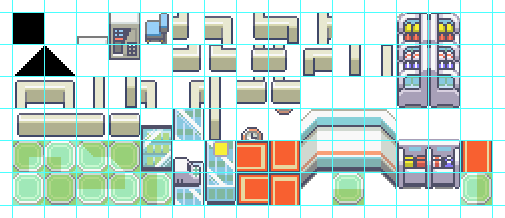
\includegraphics[width=0.8\linewidth]{tileset.png}}
    \caption{Tileset utilizzato con suddivisione in griglia}
    \label{fig:tileset}
\end{figure}

Le mappe sono state studiate appositamente ponendo particolare attenzione alle proporzioni degli ambienti e agevolate nella loro realizzazione con l'ausilio di un software apposito.

\subsubsection{TILED}
Tiled è un software open-source studiato per la costruzione di livelli focalizzato sulla semplicità di utilizzo.[cite:https://www.mapeditor.org/]
Questo ci ha permesso di creare rapidamente delle mappe ed apportare modifiche in corso d'opera efficientemente per poi esportare il lavoro realizzato in un formato utile alla successiva visualizzazione.

\subsubsection{Visualizzazione}
La lettura e la visualizzazione del terreno sulla griglia nativa di Mesa ha comportato modifiche sostanziali in alcuni file del framework.
In aggiunta, sono state applicate alcune ottimizzazioni per ridurre la complessità del processo di aggiornamento della griglia ad ogni step.

\section{Implementazione}

\subsection{Diagramma delle classi}
Il diagramma illustrato in \cref{fig:class-diagram} presenta la struttura del codice del progetto. Il framework Mesa fornisce alcune classi da estendere per agevolare la scrittura del modello, permettendo di dover implementare la sola logica applicativa.

\begin{figure}[H]
    \makebox[\textwidth][c]{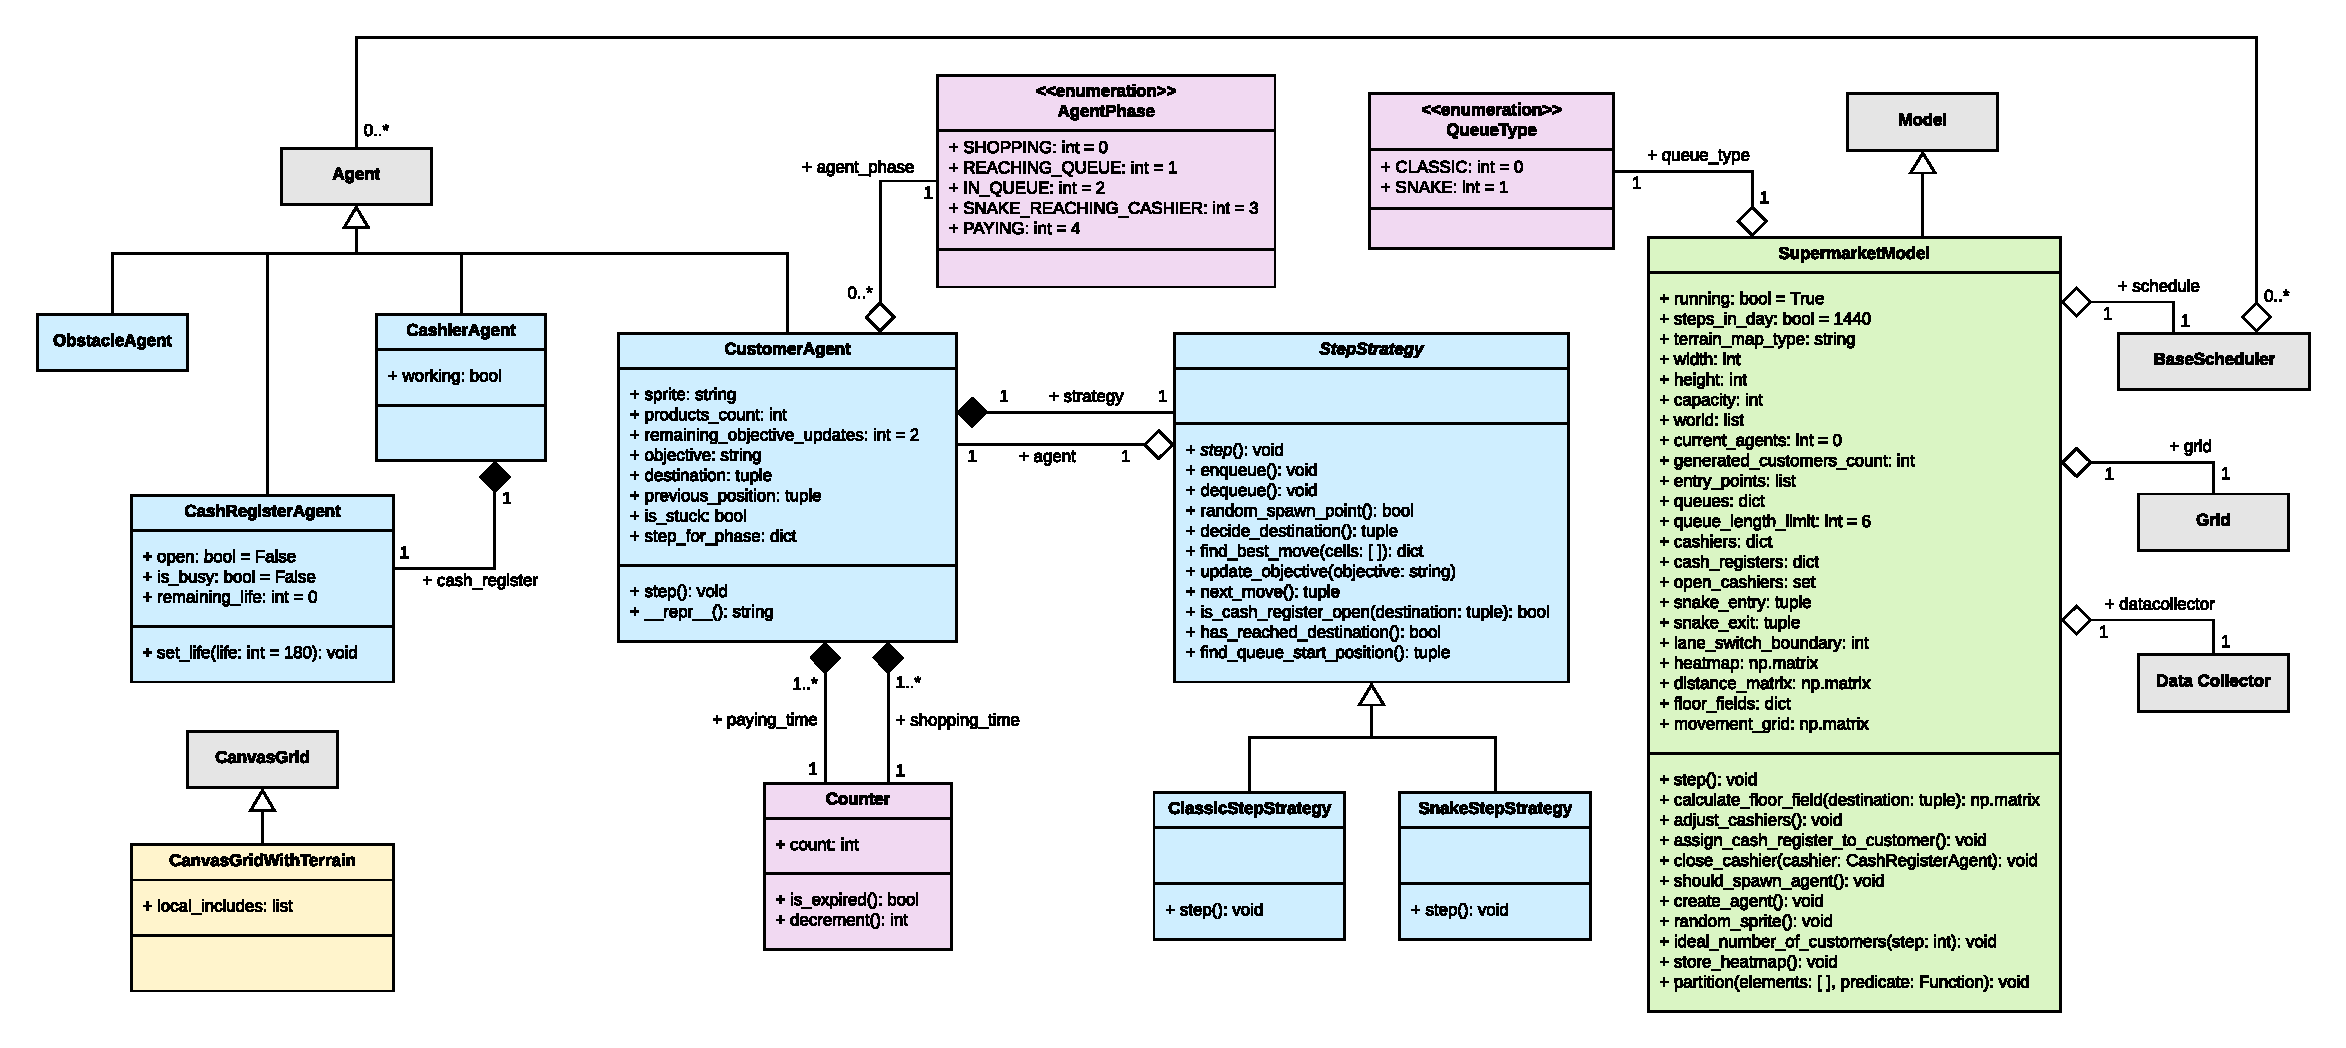
\includegraphics[width=1.45\linewidth]{class-diagram-colored.pdf}}
    \caption{Diagramma delle classi}
    \label{fig:class-diagram}
\end{figure}

\noindent
Per semplificare la comprensibilità dello schema, sono stati inclusi esclusivamente i dettagli delle classi da noi implementate, evidenziandole con colori diversi di sfondo in base alla propria finalità:
\begin{itemize}
    \item \textbf{Grigio:} classi base per permettere la simulazione di un modello attraverso Mesa.
    \item \textbf{Viola:} classi di servizio ed enumerazioni.
    \item \textbf{Azzurro:} definisce gli agenti e le strategie di movimento.
    \item \textbf{Verde:} classe principale del modello; coordina l'interazione tra Mesa e gli agenti.
    \item \textbf{Giallo:} visualizzazione e controllo dell'interazione tramite interfaccia web.
\end{itemize}

\subsection{Strategy Pattern}
La gestione di due diverse tipologie di coda, a livello implementativo, presenta molte fasi in comune, tuttavia un agente dovrà comportarsi diversamente a seconda della tipologia di coda scelta.
A tale proposito, si è scelto di implementare il pattern strategy.

La dichiarazione di una classe comune \lstinline{StepStrategy} permette di astrarre i comportamenti dell'agente in sottoclassi esterne allo stesso.
Questo consente di ridurre notevolmente la complessità del codice isolando i dettagli implementativi del movimento e rende possibile la modifica a runtime del comportamento dell'agente senza la necessità di intervenire manualmente sul codice.

\section{Conclusioni}

\subsection{Confronto Risultati}

\subsection{Sviluppi Futuri}

\end{document}
